\documentclass[12pt,a4paper]{article}

%------------------------------------------------
% Packages
%------------------------------------------------
\usepackage[T1]{fontenc}
\usepackage{lmodern}
\usepackage{graphicx}
\usepackage{amsmath,amssymb}
\usepackage{siunitx}
\usepackage{geometry}
\usepackage{fancyhdr}
\usepackage{booktabs}
\usepackage{caption}
\usepackage{float}
\usepackage{subcaption}
\usepackage{array}
\usepackage{setspace}
\usepackage[hidelinks]{hyperref}
\usepackage[backend=biber,style=numeric]{biblatex}

\addbibresource{references.bib}

%------------------------------------------------
% Page layout
%------------------------------------------------
\geometry{
    top=1in,
    bottom=1.2in,
    left=1in,
    right=1in
}

\setlength{\headheight}{15pt}
\setlength{\parskip}{0.4em}
\setlength{\parindent}{0pt}

\pagestyle{fancy}
\fancyhf{}
\fancyhead[L]{Ian Cullinane}
\fancyhead[R]{Newton's Rings}
\fancyfoot[C]{\thepage}

\sisetup{
    inter-unit-product = \cdot,
    uncertainty-mode = separate,
    per-mode = symbol
}

%------------------------------------------------
% Title
%------------------------------------------------
\title{
    \Large\textbf{Investigation of Newton's Rings}\\[0.5em]
    \large PY2107 -- Experiment 5
}

\author{
    Ian Cullinane -- \textit{125413342}\\[0.5em]
    Lab Partner: Fionn Lichtsinn Doyle\\[0.5em]
    Demonstrators: Jonathan and Olivia
}

\date{23rd September 2026}

\begin{document}

\maketitle
\thispagestyle{empty}

\newpage
\tableofcontents
\newpage

%================================================
\section{Abstract}
%================================================

Newton's rings were investigated using the interference
of red light reflected from the thin film formed between
a convex lens and a flat glass plate. The experiment
aimed to determine the wavelength of the incident light
and the refractive index of water.

The radii of successive dark fringes were measured
using a travelling microscope, first with air and then
with water between the lens and the glass plate. The
squared radii were plotted against fringe order,
and linear regression was used to determine the slopes
of the two data sets.

The wavelength was determined from the slope of the
air measurements and the radius of curvature of the
lens. The refractive index of water was determined
from the ratio of the air and water slopes.

Using the scale factor applied to the recorded data, the
air-run slope gave a wavelength of
\SI{581\pm18}{nm}. The water-run slope corresponds to an
in-water wavelength of \SI{446\pm16}{nm}; the ratio of
the slopes gave $n_{\mathrm{water}}=1.30\pm0.03$. This is
consistent with the refractive index of water at
\SI{20}{\degreeCelsius} and \SI{589}{nm} within the stated
uncertainty. The residuals are within twice the propagated
measurement uncertainty. However, the recorded calibration
length and the scale factor used in the data do not agree,
so the absolute wavelength results are provisional.

\newpage

%================================================
\section{Theory}
%================================================

\subsection{Formation of Newton's Rings}

Newton's rings are a system of concentric circular
interference fringes produced when a convex lens is
placed on a flat glass plate. The space between the
curved lower surface of the lens and the glass plate
forms a thin film whose thickness increases with
distance from the point of contact.

In this experiment, monochromatic red light is
incident approximately normally on the lens and
glass plate. Some of the incident light is reflected
at the lower surface of the lens, while another
portion is transmitted through the thin film and
reflected at the glass plate. These two reflected
rays recombine and interfere.

At the lens--air interface, reflection occurs from
a region of higher refractive index to a region of
lower refractive index. There is therefore no phase
change on reflection. At the air--glass interface,
reflection occurs from a medium of lower refractive
index to a medium of higher refractive index,
resulting in a phase change of $\pi$ radians.

This phase change corresponds to an additional
optical path difference of $\lambda/2$. Consequently,
the conditions for constructive and destructive
interference are reversed relative to the case in
which neither reflected ray undergoes a phase change.

The interference pattern consists of alternating
bright and dark circular fringes. The thickness of
the air film increases with distance from the centre,
causing the path difference to vary with radius. \cite{hecht}

\subsection{Geometrical Relationship}

Let $R$ be the radius of curvature of the lens,
$r_n$ the radius of the $n$th dark ring, and $t$
the thickness of the film at that radius.

From the geometry of the lens,

\[
R^2=(R-t)^2+r_n^2.
\]

Expanding,

\[
R^2=R^2-2Rt+t^2+r_n^2.
\]

Rearranging gives

\[
r_n^2=2Rt-t^2.
\]

Since the thickness of the film is very small
compared with the radius of curvature, the term
$t^2$ can be neglected. Hence,

\[
\boxed{r_n^2\simeq 2Rt}.
\]

The optical path difference between the two
reflected rays is approximately $2t$ for
near-normal incidence.

\begin{figure}[h]
    \centering
    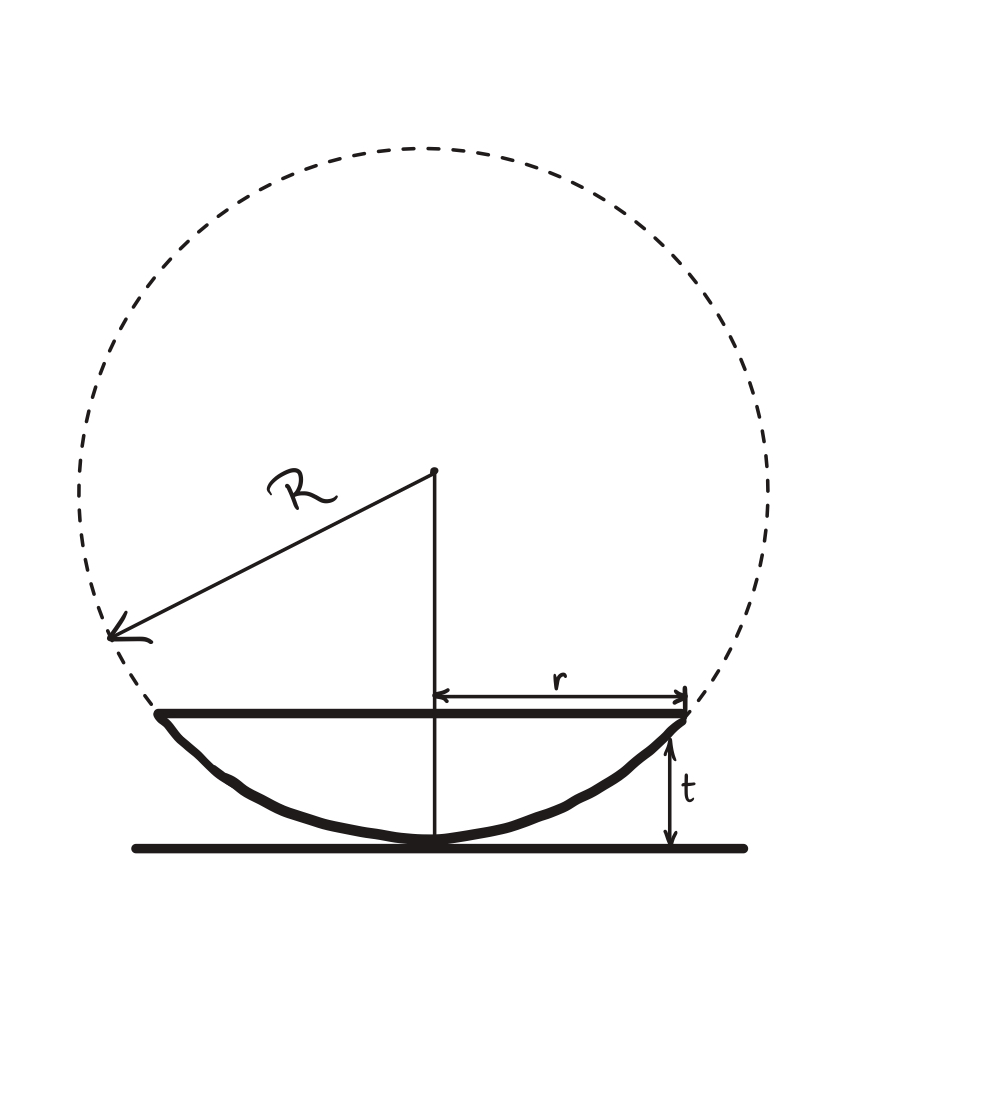
\includegraphics[width=0.6\textwidth]{images/Lens_geometry.jpg}
    \caption{Geometry of the lens and air film in Newton's Rings experiment.}
    \label{fig:lens_geometry}
\end{figure}

\subsection{Condition for Dark Fringes}

Because one of the reflected rays undergoes a
phase change of $\pi$, destructive interference
in reflected light occurs when

\[
2t=n\lambda,
\]

where $n=0,1,2,\ldots$ is the order of the dark
fringe and $\lambda$ is the wavelength of the
incident light.

Substituting $t=r_n^2/(2R)$ gives

\[
\frac{r_n^2}{R}=n\lambda.
\]

Therefore,

\begin{equation}
    \boxed{
    r_n^2=nR\lambda
    }.
    \label{eq:governing_equation}
\end{equation}

This predicts a linear relationship between
the squared radius and the fringe order.

\subsection{Determination of the Wavelength}

Equation~\ref{eq:governing_equation} can be written as

\[
\frac{r_n^2}{R}=S_{\mathrm{air}}n,
\]

where the slope of the graph of $\frac{r_n^2}{R}$ against
$n$ is

\[
\boxed{S_{\mathrm{air}}=\lambda}.
\]

The slope is obtained from a least-squares linear
fit to the measured values of $\frac{r_n^2}{R}$ and their
corresponding fringe orders.

\subsection{Determination of the Refractive Index
of Water}

When the air film is replaced by water, the
wavelength within the water becomes

\[
\lambda_{\mathrm{water}}
=\frac{\lambda}{n_{\mathrm{water}}},
\]

where $n_{\mathrm{water}}$ is the refractive index
of water relative to air.

The dark-fringe condition becomes

\[
2n_{\mathrm{water}}t=n\lambda.
\]

Using the geometrical relationship
$r_n^2\simeq 2Rt$,

\[
\ r_n^2
\ =Rn\frac{\lambda}{n_{\mathrm{water}}}.
\]

Therefore,

\begin{equation}
\boxed{
\frac{r_n^2}{R}
=\frac{\lambda}{n_{\mathrm{water}}}n
}.
\label{eq:water_slope}
\end{equation}

Defining the slope of the water graph as
$S_{\mathrm{water}}$ gives

\[
S_{\mathrm{water}}
=\frac{\lambda}{n_{\mathrm{water}}}.
\]

Dividing the air slope by the water slope
eliminates both the radius of curvature and
the wavelength:

\begin{equation}
\boxed{
n_{\mathrm{water}}  
=\frac{S_{\mathrm{air}}}{S_{\mathrm{water}}}
}.
\label{eq:ref_index}
\end{equation}

This provides an independent determination
of the refractive index without requiring
a separate measurement of the radius of
curvature.

\newpage

%================================================
\section{Experimental Procedure}
%================================================

\subsection{Apparatus}

The apparatus consisted of a convex lens, a
flat glass plate, a red light source, a glass
reflector inclined at approximately
\SI{45}{\degree}, a travelling microscope
with a camera, a translation stage with a
vernier scale, and a spherometer as seen in Fig~\ref{fig:apparatus} and Fig~\ref{fig:spherometer}.

The lens was placed on the glass plate to
produce the thin film required for Newton's
rings. The reflected interference pattern
was observed using the microscope and camera
system. \cite{py2107}

\begin{figure}[H]
    \centering
    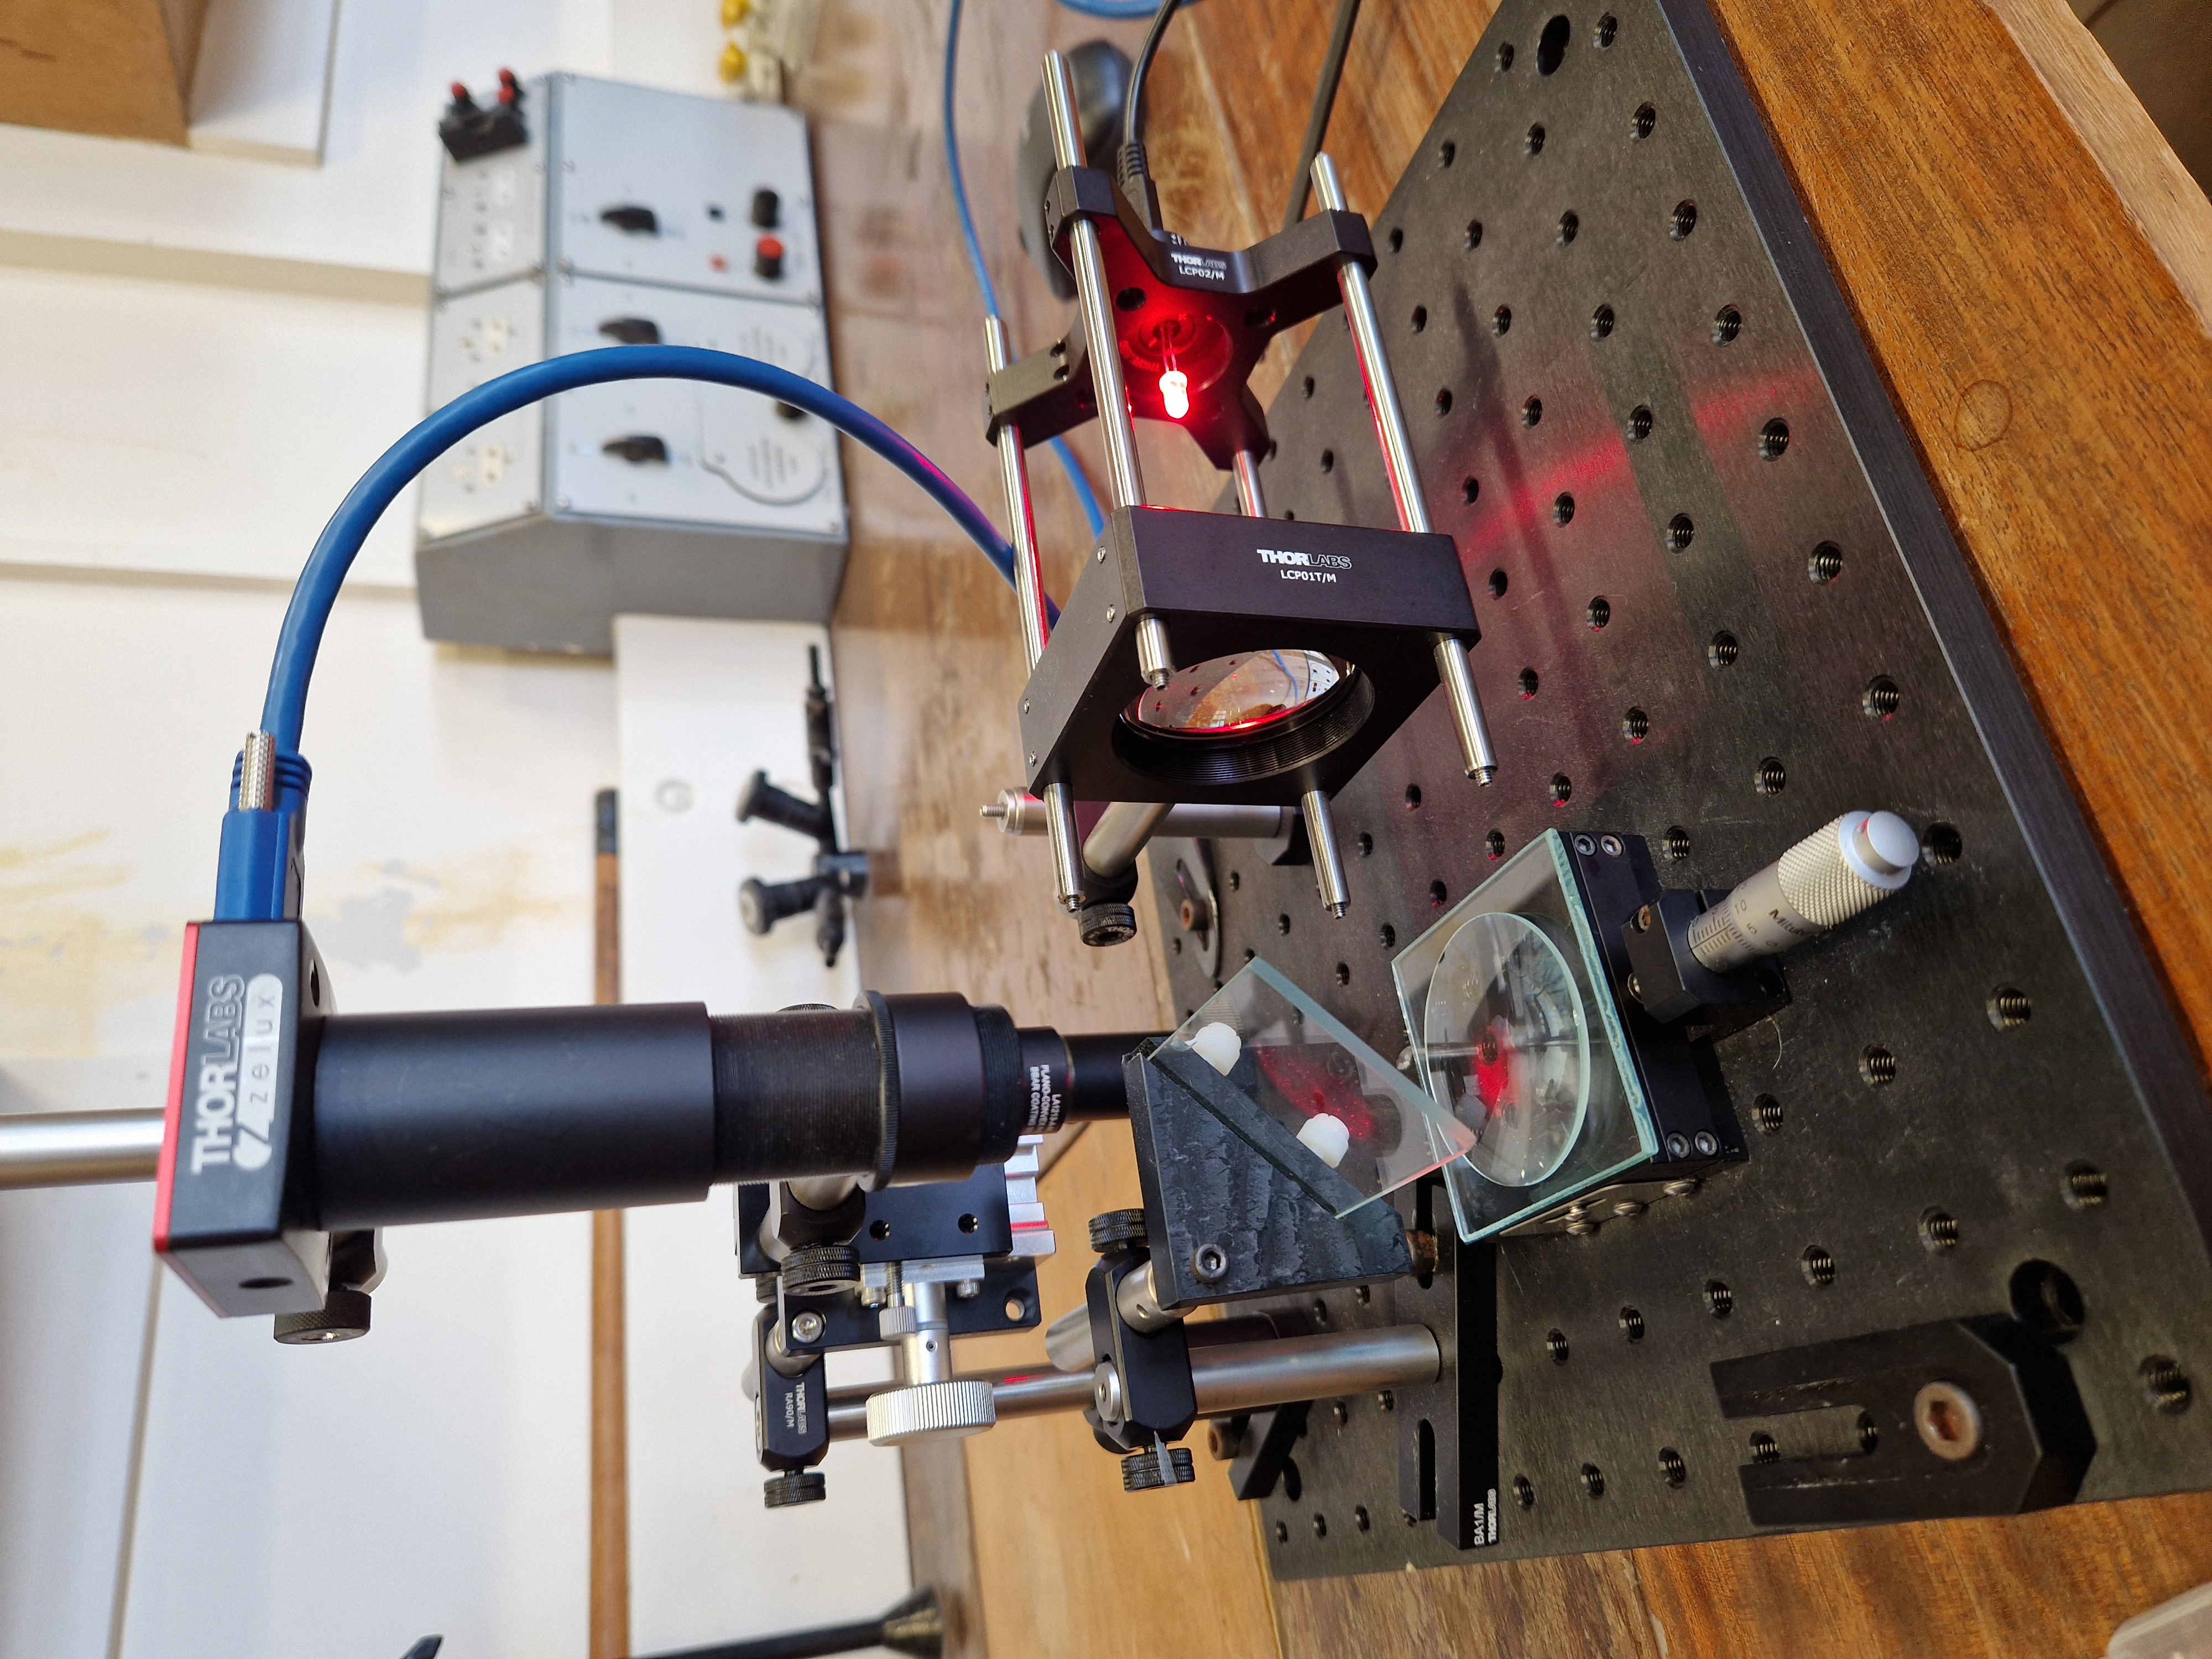
\includegraphics[width=0.5\linewidth, angle=-90]{images/Apparatus.jpg}
    \caption{Apparatus used for this experiment}
    \label{fig:apparatus}
\end{figure}

\begin{figure}[H]
    \centering
    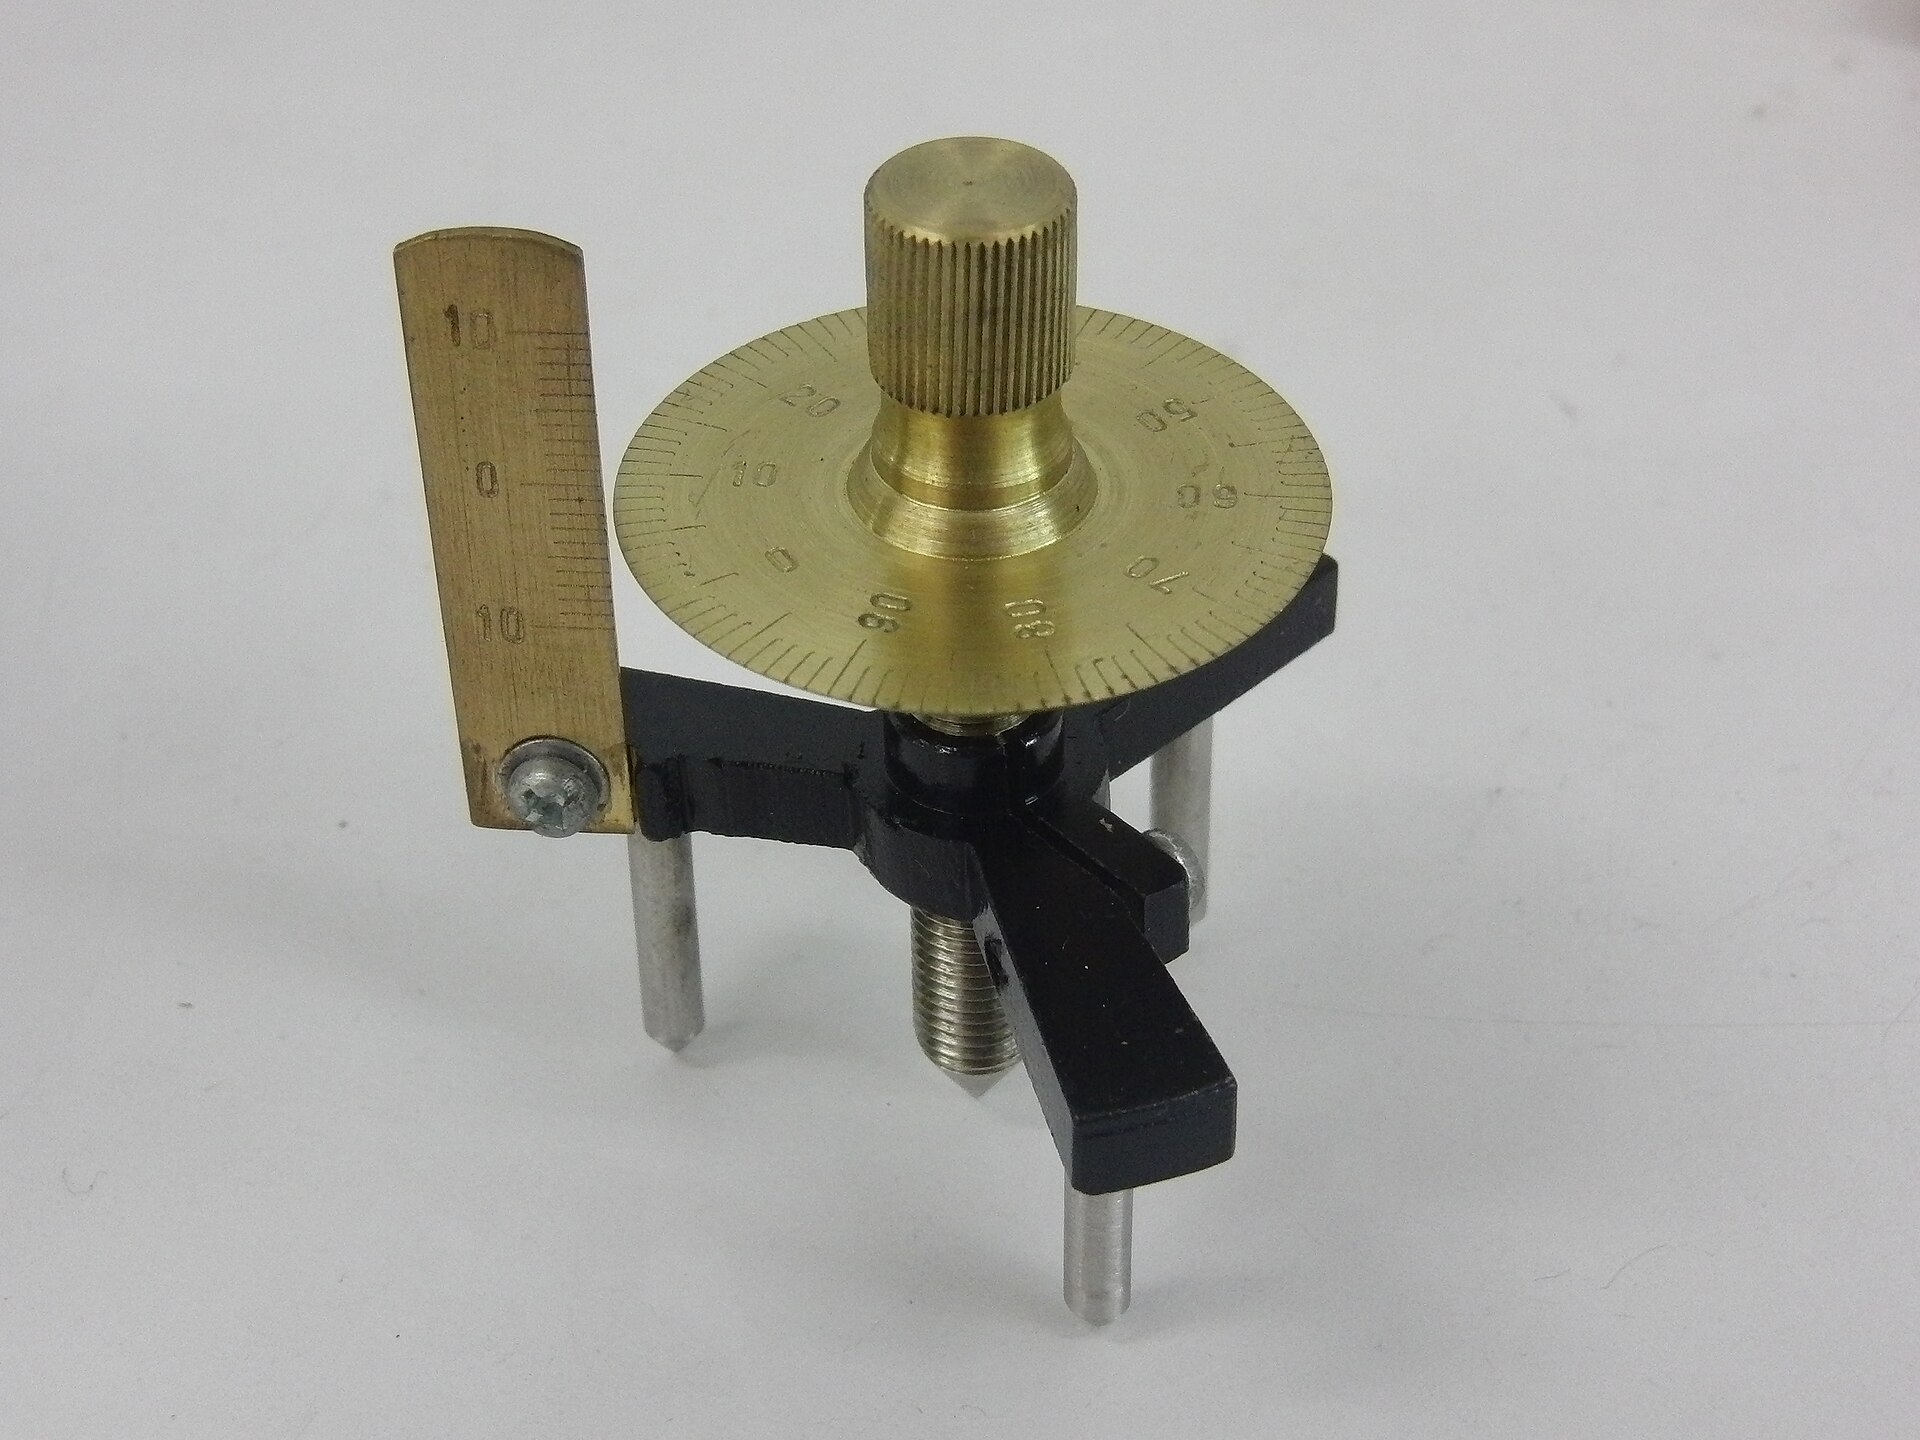
\includegraphics[width=0.5\linewidth]{images/spherometer.png}
    \caption{Spherometer as used in this experiment}
    \label{fig:spherometer}
\end{figure}

\subsection{Observation of the Rings}

The light source and camera were switched on, and the microscope was focused until a clear pattern of concentric rings was visible. The camera exposure was adjusted to obtain sufficient contrast between the dark and bright fringes.

The calibration was then completed according to the procedure below.

The centre of the pattern was identified, and the dark rings were numbered consecutively. The first visible dark ring was assigned order $n=1$ as seen in Fig~\ref{fig:newtons_rings_slice}. The dark central region was not counted as the first ring.

\begin{figure}[H]
    \centering
    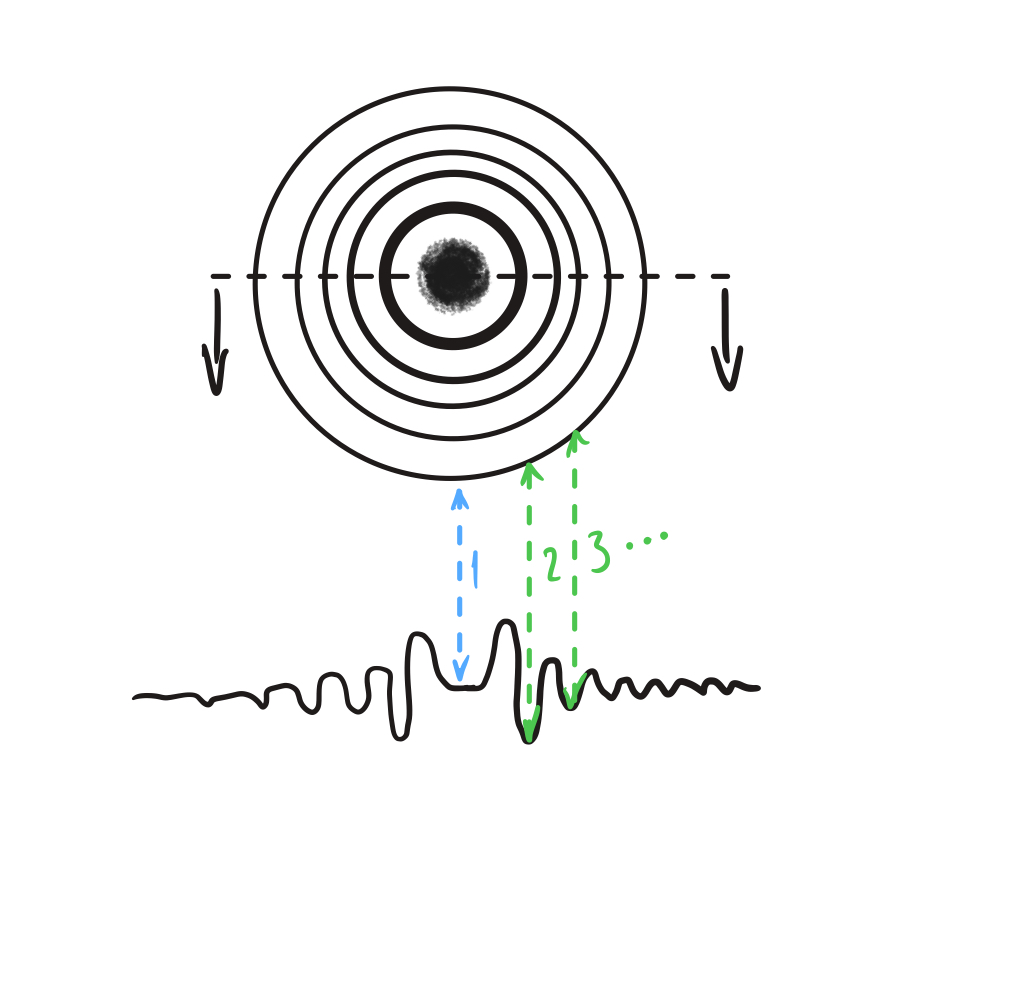
\includegraphics[width=0.5\linewidth]{images/Projection.jpg}
    \caption{Newton's rings as ordered in the experiment}
    \label{fig:newtons_rings_slice}
\end{figure}

\subsection{Calibration and Measurement in Air}

The travelling microscope was calibrated by relating the displacement of the translation stage, measured using its vernier scale, to the corresponding displacement in the camera image. A fringe was lined up with the bottom of the image then moved to the top. The camera image height was $1080$ pixels. The scale factor used to calculate the tabulated radii was

\begin{equation}
PD = \frac{L_{m}}{L_p},
\label{eq:pixel density}
\end{equation}
We get,
\[
    PD = \frac{0.0037}{1080} = 3.12\times10^{-6}m/p.
\]

The ring positions were recorded in pixels. The displacement of each ring from the central reference position was calculated.

The air measurements were completed before introducing water between the lens and the glass plate.

\subsection{Measurement with Water}

After the air measurements were completed, small drops of water were introduced at the
edges of the glass plate. The water was allowed to spread into the gap between the
lens and the plate.

The dark-ring radii were measured again using the same microscope and calibration
procedure. The contrast of the rings was lower after the introduction of water,
increasing the difficulty of locating their boundaries.

\subsection{Radius of Curvature}

The radius of curvature of the lens was determined using a spherometer.

The radius of curvature was calculated from the spherometer geometry using the average $IPD$ (inter-pin distance), measured using vernier calipers, and the measured sagitta. The radius of the pin $l$ was calculated as

\[
2l = IPD\sin\phi + \frac{IPD}{2}\tan\phi.
\]

The radius of curvature was then calculated as

\[
R = \frac{l^2+h^2}{2h}
\]

The measured sagitta was

\[
h=\SI{1.003 \pm 0.0005}{mm}.
\]

and IPD was taken as the average,

\[
IPD = \SI{0.0397 \pm 0.007}{m}.
\]

giving us

\[
R=\SI{0.2625\pm 0.008}{m}.
\]

\begin{figure}[H]
    \centering
    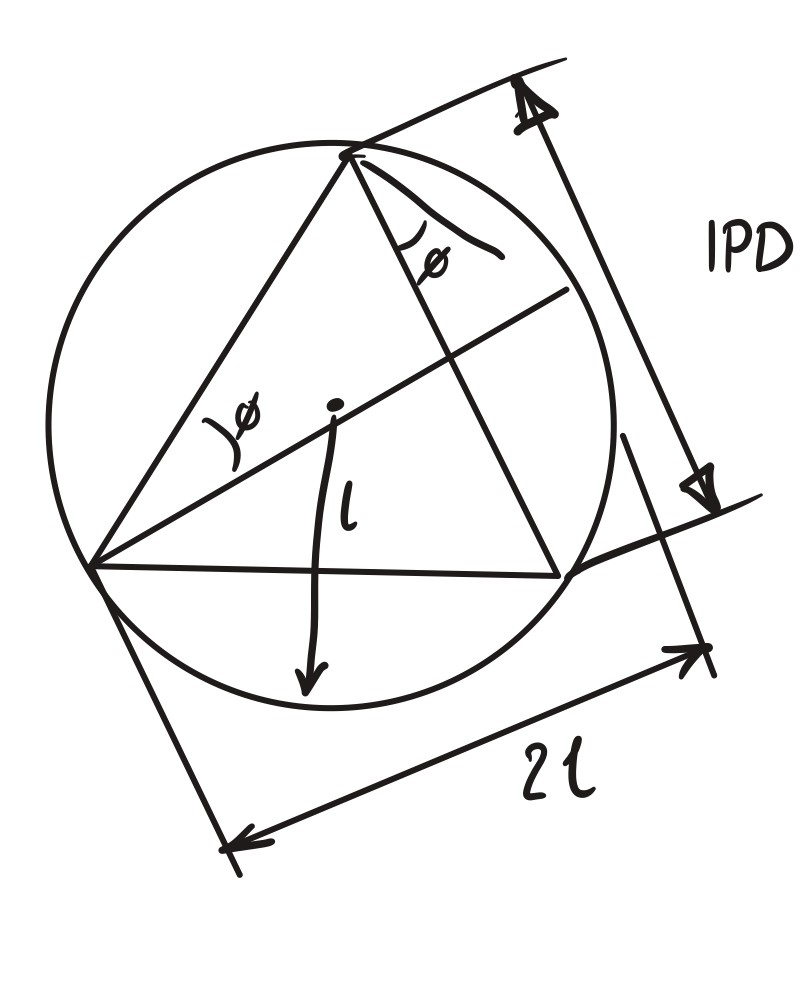
\includegraphics[width=0.5\linewidth]{images/Spherometer_geometry.jpg}
    \caption{Geometry of the spherometer pins}
    \label{fig:spherometer_geometry}
\end{figure}

\newpage

%================================================
\section{Results}
%================================================

\begin{table}[H]
    \centering
    \caption{Recorded data for the run with air.}
    \label{tab:air}
    \small
    \begin{tabular}{cccc}
    \toprule
    $n$ & $p$ (pixels) & $\Delta p$ (pixels)
    & $r_n^2$ (\si{m^2})\\
    \midrule
    0  & 720  & 0   & --\\
    1  & 828  & 108 & $1.13569\times10^{-7}$\\
    2  & 886  & 166 & $2.68305\times10^{-7}$\\
    3  & 930  & 210 & $4.29389\times10^{-7}$\\
    4  & 961  & 241 & $5.65518\times10^{-7}$\\
    5  & 992  & 272 & $7.20361\times10^{-7}$\\
    6  & 1019 & 299 & $8.70472\times10^{-7}$\\
    7  & 1046 & 326 & $1.03478\times10^{-6}$\\
    8  & 1069 & 349 & $1.18594\times10^{-6}$\\
    9  & 1090 & 370 & $1.33296\times10^{-6}$\\
    10 & 1112 & 392 & $1.49618\times10^{-6}$\\
    11 & 1133 & 413 & $1.66078\times10^{-6}$\\
    12 & 1151 & 431 & $1.80870\times10^{-6}$\\
    13 & 1169 & 449 & $1.96293\times10^{-6}$\\
    14 & 1184 & 464 & $2.09627\times10^{-6}$\\
    15 & 1199 & 479 & $2.23400\times10^{-6}$\\
    16 & 1214 & 494 & $2.37611\times10^{-6}$\\
    17 & 1233 & 513 & $2.56240\times10^{-6}$\\
    18 & 1248 & 528 & $2.71444\times10^{-6}$\\
    19 & 1264 & 544 & $2.88144\times10^{-6}$\\
    20 & 1277 & 557 & $3.02080\times10^{-6}$\\
    21 & 1290 & 570 & $3.16346\times10^{-6}$\\
    22 & 1306 & 586 & $3.34355\times10^{-6}$\\
    23 & 1319 & 599 & $3.49354\times10^{-6}$\\
    24 & 1330 & 610 & $3.62303\times10^{-6}$\\
    25 & 1342 & 622 & $3.76698\times10^{-6}$\\
    26 & 1355 & 635 & $3.92609\times10^{-6}$\\
    27 & 1363 & 643 & $4.02563\times10^{-6}$\\
    28 & 1378 & 658 & $4.21565\times10^{-6}$\\
    \bottomrule
    \end{tabular}
\end{table}

\begin{table}[H]
\centering
\caption{Recorded data for the run with water.}
\label{tab:water}
\small
\begin{tabular}{cccc}
\toprule
$n$ & $p$ (pixels) & $\Delta p$ (pixels) & $r_n^2$ (\si{m^2})\\
\midrule
0 & 803 & 0 & -- \\
1 & 926 & 123 & $1.47307\times10^{-7}$ \\
2 & 964 & 161 & $2.52385\times10^{-7}$ \\
3 & 1000 & 197 & $3.77872\times10^{-7}$ \\
4 & 1029 & 226 & $4.97312\times10^{-7}$ \\
5 & 1056 & 253 & $6.23237\times10^{-7}$ \\
6 & 1076 & 273 & $7.25667\times10^{-7}$ \\
7 & 1100 & 297 & $8.58866\times10^{-7}$ \\
8 & 1116 & 313 & $9.53896\times10^{-7}$ \\
9 & 1136 & 333 & $1.07969\times10^{-6}$ \\
\bottomrule
\end{tabular}
\end{table}

For both runs, the radii were calculated from the measured displacement using $r_n=\Delta p\,PD$ and $r_n^2=(\Delta p\,PD)^2$. The tabulated squared radii are based on the scale factor stated in the analysis data; the calibration discrepancy described above therefore applies to these values as well.

\newpage

%================================================
\section{Analysis}
%================================================

\subsection{Linear Regression}

The theoretical relationship for dark
fringes is

\[
r_n^2=Rn\lambda.
\]

A linear regression was performed on
the squared radii as a function of
fringe order:

\[
\frac{r_n^2}{R}=Sn+b,
\]

where $S$ is the fitted slope and $b$
is the intercept.

The weighted regression slopes and their fit uncertainties were

\[
S_{\mathrm{air}}
=(5.81\pm0.03)\times10^{-7}\ \si{m}
\]
and

\[
S_{\mathrm{water}}
=(4.46\pm0.08)\times10^{-7}\ \si{m}.
\]

Because the plotted quantity is $r^2/R$, these slopes have units of metres. The air slope gives the wavelength in air, while the water slope gives the wavelength in water, $\lambda_{\mathrm{water}}=\lambda_{\mathrm{air}}/n_{\mathrm{water}}$.

The coefficients of determination were reported as

\[
R_{\mathrm{air}}^2=0.99983
\]

and

\[
R_{\mathrm{water}}^2=0.99943.
\]

These values indicate a strong overall linear relationship, but they do not by themselves establish that the residuals are random or that the measurement uncertainties are realistic.

\begin{figure}[H]
    \centering
    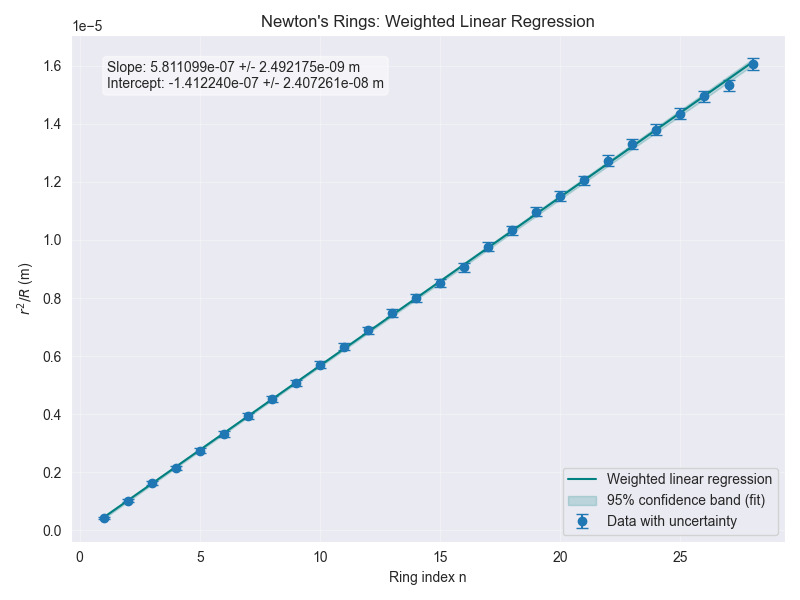
\includegraphics[width=0.8\textwidth]{images/newtons_rings_regression_air.png}
    \caption{Linear regression of $r^2/R$ against fringe order for the air run.}
    \label{fig:regression_air}
\end{figure}

\begin{figure}[H]
    \centering
    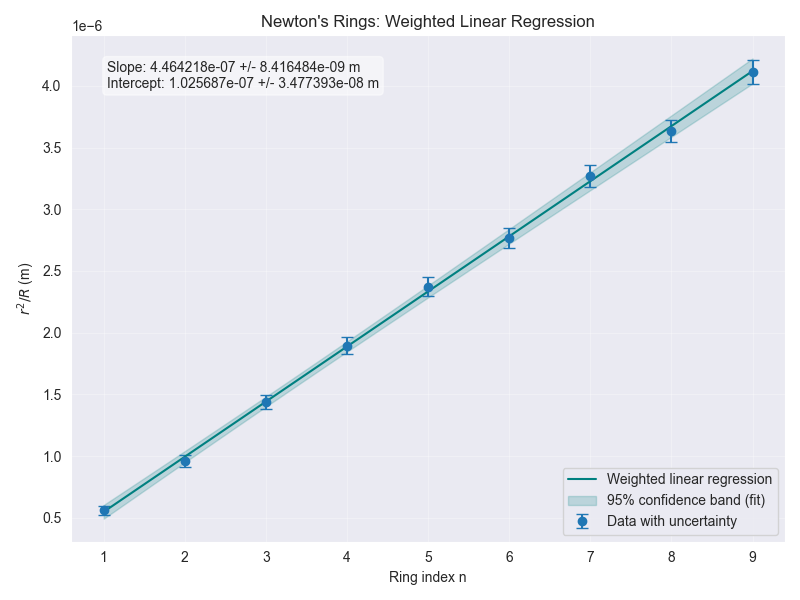
\includegraphics[width=0.8\textwidth]{images/newtons_rings_regression_water.png}
    \caption{Linear regression of $r^2/R$ against fringe order for the water run.}
    \label{fig:regression_water}
\end{figure}

The standardised residuals, calculated as
$(y_n-y_{n,\mathrm{fit}})/\sigma_{y_n}$, are shown in Figures~\ref{fig:residuals_air} and \ref{fig:residuals_water}. Here $y_n=r_n^2/R$ and $\sigma_{y_n}$ is propagated from the assumed four-pixel uncertainty in ring position.

\begin{figure}[H]
    \centering
    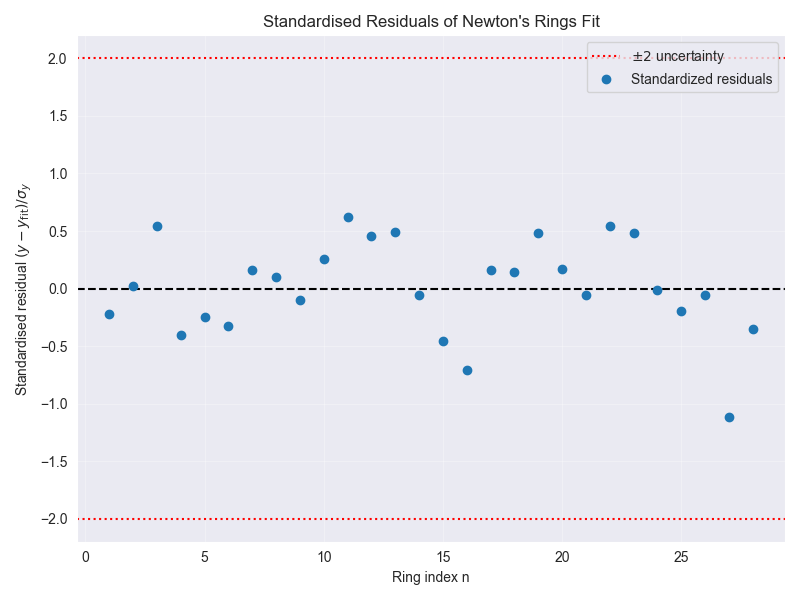
\includegraphics[width=0.8\textwidth]{images/residuals_air.png}
    \caption{Standardised residuals for the air run. The dotted lines mark $\pm2$ propagated standard uncertainties.}
    \label{fig:residuals_air}
\end{figure}

\begin{figure}[H]
    \centering
    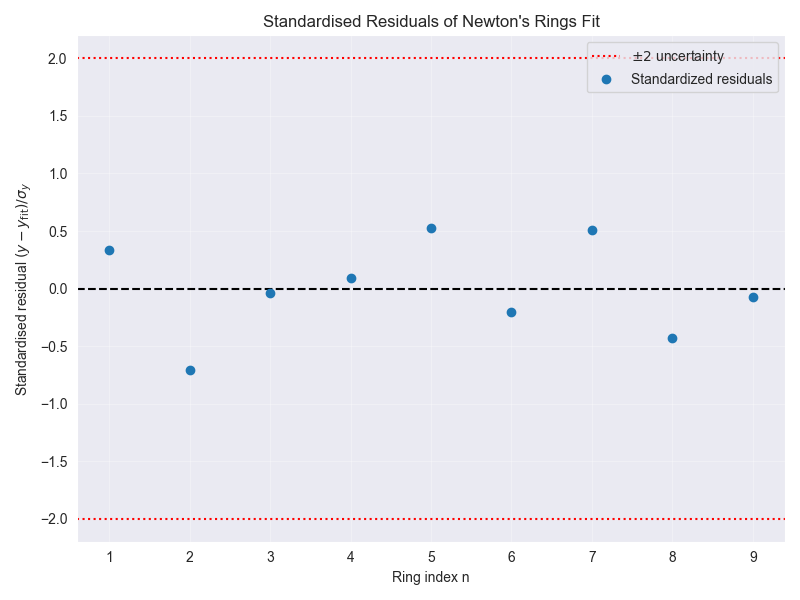
\includegraphics[width=0.8\textwidth]{images/residuals_water.png}
    \caption{Standardised residuals for the water run. The dotted lines mark $\pm2$ propagated standard uncertainties.}
    \label{fig:residuals_water}
\end{figure}

\subsection{Refractive Index of Water}

From Equation~\ref{eq:ref_index},

\[
n_{\mathrm{water}}
=\frac{S_{\mathrm{air}}}{S_{\mathrm{water}}}.
\]

Substituting the fitted slopes,

\[
n_{\mathrm{water}}
=
\frac{5.81\times10^{-7}}
{4.46\times10^{-7}}.
\]

Hence,

\[
\boxed{n_{\mathrm{water}}=1.30\pm0.03}.
\]

\newpage

%================================================
\section{Uncertainty Analysis}
%================================================

\subsection{Uncertainty in the Wavelength}

The wavelength in air is obtained directly from the fitted air slope, $\lambda_{\mathrm{air}}=S_{\mathrm{air}}$. Treating the fit and curvature uncertainties as independent, uncertainty propagation gives

\[
\left(\frac{\sigma_\lambda}{\lambda}\right)^2
=
\left(\frac{\sigma_{S_{\mathrm{air}}}}
{S_{\mathrm{air}}}\right)^2
+
\left(\frac{\sigma_R}{R}\right)^2.
\]

\begin{equation}
    \sigma_{\lambda} = \lambda \sqrt{\left(\frac{\sigma_{S_{\mathrm{air}}}}{S_{\mathrm{air}}}\right)^2 + \left(\frac{\sigma_R}{R}\right)^2}
    \label{eq:uncertainty_lambda}
\end{equation}

The radius of curvature used in the fit was

\[
R=\SI{0.2625}{m}
\]

with an uncertainty of approximately

\[
\sigma_R=\SI{0.008}{m}.
\]

The relative uncertainty in the radius
is therefore

\[
\frac{\sigma_R}{R}
=
\frac{0.008}{0.2625}
=0.0305.
\]

The relative uncertainty of the slope was

\[
\frac{\sigma_{S_{\mathrm{air}}}}{S_{\mathrm{air}}}=0.0043.
\]

Using Equation~\ref{eq:uncertainty_lambda}, the uncertainty in the wavelength is then

\[
\sigma_\lambda\approx\SI{18}{nm}.
\]

The final wavelength result is

\[
\boxed{
\lambda_{\mathrm{air}}=(581\pm18)\ \si{nm}
}.
\]

The principal contributions to the
uncertainty are the determination of
the radius of curvature and the
measurement of the ring radii.

Applying the same propagation to the
water-run slope gives the wavelength
within the water film:

\[
\lambda_{\mathrm{water}}=(446\pm16)\ \si{nm}.
\]

\subsection{Uncertainty in the Refractive Index}

The refractive index is determined
from the ratio

\[
n_{\mathrm{water}}
=\frac{S_{\mathrm{air}}}{S_{\mathrm{water}}}.
\]

Assuming independent fit uncertainties
for the two slopes,

\[
\left(\frac{\sigma_n}{n_{\mathrm{water}}}\right)^2
=
\left(\frac{\sigma_{S_{\mathrm{air}}}}
{S_{\mathrm{air}}}\right)^2
+
\left(\frac{\sigma_{S_{\mathrm{water}}}}
{S_{\mathrm{water}}}\right)^2
\]

Using the uncertainties of the two linear fits gives

\[
\sigma_n\approx0.03.
\]

Thus,

\[
\boxed{
n_{\mathrm{water}}=1.30\pm0.03
}.
\]

The radius of curvature does not contribute to this uncertainty because it cancels when the two slopes are divided.

Similarly, a common calibration factor cancels from the ratio, provided that the same calibration was used for both the air and water measurements.

\newpage

%================================================
\section{Discussion}
%================================================

\subsection{Wavelength}

The air-run slope gives
$\lambda_{\mathrm{air}}=(581\pm18)\ \si{nm}$, consistent
with the red source used in the experiment. The
water-run slope corresponds instead to the wavelength
within the water film,
$\lambda_{\mathrm{water}}=(446\pm16)\ \si{nm}$. This value
is shorter, as expected for light propagating through
a medium with refractive index greater than one. It is
not an independent estimate of the source's wavelength
in air.

\subsection{Refractive Index}

The refractive index obtained from
the slope ratio was

\[
n_{\mathrm{water}}=1.30 \pm 0.03.
\]

At approximately \SI{20}{\degreeCelsius} and \SI{589}{nm}, the refractive index of water is about 1.333\cite{daimon2007}. The measured value is lower by about 0.03, or roughly one standard uncertainty. This is close agreement, although the central reference value lies just outside the stated one-standard-uncertainty interval. The comparison should be treated cautiously because the calibration uncertainty and other systematic effects may not be fully represented.

The remaining uncertainty is consistent with limitations in locating the ring boundaries and centre, as well as possible non-uniform filling of the gap by water. The lower contrast of the water fringes makes their positions more difficult to determine.

\subsection{Residuals}

Residuals are shown in units of their propagated measurement uncertainty, so values within $\pm2$ are within twice the assumed uncertainty. For the weighted linear fits, the standardised residuals range from $-1.11$ to $0.62$ for air and from $-0.71$ to $0.53$ for water. None exceeds $2$ in magnitude. The air residuals are not perfectly patternless, and the water run contains only nine rings, so these plots provide a limited diagnostic rather than proof that the model and uncertainty estimates are complete. In particular, the four-pixel position uncertainty is an assumption and should be checked against repeated measurements or image-based uncertainty estimates.

\subsection{Sources of Experimental Error}

Several factors may have contributed to uncertainty in the measured ring radii.

Firstly, identifying the exact centre of the Newton's rings pattern is difficult because the central dark region has a finite size. An error in the reference position introduces an offset in the displacement measurements.

Secondly, the dark-ring boundaries were not perfectly sharp. This was particularly important for the water measurements, where the contrast was reduced.

Thirdly, errors in the calibration of the microscope affect the absolute wavelength calculation. However, a common calibration factor cancels from the ratio used to calculate the refractive index.

The assumption that water uniformly
fills the gap between the lens and
glass plate may also introduce
systematic error. If air bubbles
remain or the water film is not
uniform, the effective optical
path difference may differ from
the theoretical model.

Finally, uncertainty in the
spherometer measurement affects
the radius of curvature and
therefore the calculated wavelength.
It does not affect the refractive
index obtained from the ratio
of slopes.

\subsection{Improvements}

The accuracy of the experiment
could be improved by measuring
each ring on both sides of the
centre and using half the
separation as its radius. Repeated
measurements would help quantify
the position uncertainty and
reduce sensitivity to an
incorrectly identified centre.

The calibration should be performed
over the largest practical
displacement using the translation
stage and repeated to check
its reproducibility.

For the water measurements,
care should be taken to ensure
that the water spreads uniformly
beneath the lens and that air
bubbles are removed.

Improved illumination and image
contrast would also make the
ring boundaries easier to identify.

The uncertainty in the lens radius
could be reduced by taking several
spherometer measurements at
different positions and using
their mean value.

\newpage

%================================================
\section{Conclusion}
%================================================

Newton's rings were investigated
using the interference of red
light reflected from a thin film
between a convex lens and a
glass plate.

The squared radii of the
dark fringes were plotted against
their orders for both air and
water. The resulting slopes were
used to determine the wavelength
of the incident light and the
refractive index of water.

The air-run slope gave the source
wavelength as

\[
\boxed{
\lambda_{\mathrm{air}}=(581\pm18)\ \si{nm}
}.
\]

\[
\boxed{
\lambda_{\mathrm{water}}=(446\pm16)\ \si{nm}
}.
\]

The refractive index of water
was determined from the ratio
of the air and water slopes:

\[
\boxed{
n_{\mathrm{water}}=1.30\pm0.03
}.
\]

The air wavelength is consistent
with the red region of the visible
spectrum. The in-water wavelength
is shorter, as expected, and the
measured refractive index is close
to the reference value. The
standardised residuals remain
within $\pm2$ for the assumed
position uncertainty, although
the calibration discrepancy means
that the absolute wavelengths
remain provisional.

The experiment demonstrated
the relationship between
interference fringe radii
and order, and showed how
the introduction of a medium
with a higher refractive index
changes the dimensions of
the interference pattern.

%================================================
\section{References}
%================================================

\printbibliography[heading=none]

\newpage

%================================================
\appendix
\section{Derivation of the Newton's Rings Equations}
%================================================

\subsection{Geometrical Relationship}

For a lens of radius of curvature
$R$, the radius of a ring $r$
and the film thickness $t$
are related by

\[
R^2=(R-t)^2+r^2.
\]

Expanding and simplifying,

\[
r^2=2Rt-t^2.
\]

For $t\ll R$, the $t^2$ term
is negligible:

\[
r^2\simeq2Rt.
\]

Therefore,

\[
t\simeq\frac{r^2}{2R}.
\]

\subsection{Dark-Ring Radius}

For reflected light, one of
the two rays undergoes a
phase change of $\pi$.
The condition for destructive
interference is

\[
2t=n\lambda.
\]

Substituting the geometrical
expression for $t$,

\[
2\left(\frac{r_n^2}{2R}\right)
=n\lambda.
\]

Hence,

\[
r_n^2=nR\lambda.
\]

Since $D_n=2r_n$,

\[
D_n^2=4r_n^2.
\]

Therefore,

\[
\boxed{D_n^2=4Rn\lambda}.
\]

\subsection{Water Film}

For water, the wavelength
within the medium is
$\lambda/n_{\mathrm{water}}$.
The dark-ring condition is

\[
2t=n\frac{\lambda}{n_{\mathrm{water}}}.
\]

Using $t=r_n^2/(2R)$,

\[
\frac{r_n^2}{R}
=\frac{n\lambda}{n_{\mathrm{water}}}.
\]

Multiplying by four,

\[
D_n^2
=\frac{4Rn\lambda}{n_{\mathrm{water}}}.
\]

For a plot of $r_n^2/R$ against
fringe order, as used in the main
analysis, the slopes are

\[
S_{\mathrm{air}}=\lambda
\]

and

\[
S_{\mathrm{water}}
 =\frac{\lambda}{n_{\mathrm{water}}}.
\]

If the plotted quantity were $r_n^2$
instead, the slopes would be
$R\lambda$ and $R\lambda/n_{\mathrm{water}}$.
For squared diameter $D_n^2=4r_n^2$,
they would be $4R\lambda$ and
$4R\lambda/n_{\mathrm{water}}$.

Dividing the equations gives

\[
\boxed{
n_{\mathrm{water}}
=\frac{S_{\mathrm{air}}}{S_{\mathrm{water}}}
}.
\]

\end{document}